
%%%%%%%%%%%%%%%%%%%%%%% file typeinst.tex %%%%%%%%%%%%%%%%%%%%%%%%%
%
% This is the LaTeX source for the instructions to authors using
% the LaTeX document class 'llncs.cls' for contributions to
% the Lecture Notes in Computer Sciences series.
% http://www.springer.com/lncs       Springer Heidelberg 2006/05/04
%
% It may be used as a template for your own input - copy it
% to a new file with a new name and use it as the basis
% for your article.
%
% NB: the document class 'llncs' has its own and detailed documentation, see
% ftp://ftp.springer.de/data/pubftp/pub/tex/latex/llncs/latex2e/llncsdoc.pdf
%
%%%%%%%%%%%%%%%%%%%%%%%%%%%%%%%%%%%%%%%%%%%%%%%%%%%%%%%%%%%%%%%%%%%


\documentclass[runningheads,a4paper]{llncs}

\usepackage{amssymb}
\setcounter{tocdepth}{3}
\usepackage{graphicx}
\usepackage{times}
%\usepackage{cite}
%\usepackage{subfigure}
\usepackage{amsmath}
\usepackage{amssymb}
\usepackage{verbatim}


%\newtheorem{property}{\textbf{Property}}


\begin{document}




\mainmatter  % start of an individual contribution

% first the title is needed
\title{Analyzing Coopetition Strategies of Services within Communities}

% a short form should be given in case it is too long for the running head
\titlerunning{Lecture Notes in Computer Science}

% the name(s) of the author(s) follow(s) next
%
% NB: Chinese authors should write their first names(s) in front of
% their surnames. This ensures that the names appear correctly in
% the running heads and the author index.
%

\author{Babak Khosravifar$^1$
\and Mahsa Alishahi$^1$ \and Ehsan Khosrowshahi Asl$^1$ \and Jamal
Bentahar$^1$\and Rabeb Mizouni$^2$\and Hadi Otrok$^2$}

%

% (feature abused for this document to repeat the title also on left hand pages)

% the affiliations are given next; don't give your e-mail address
% unless you accept that it will be published


\institute{$^1$Concordia University, Canada, $^2$Khalifa University, UAE\\
$b\_khosr@encs.concordia.ca$, $m\_ali@encs.concordia.ca$, $e\_khosr@encs.concordia.ca$,\\$bentahar@ciise.concordia.ca$,
$rabeb.mizouni@kustar.ac.ae$,$hadi.otrak@kustar.ac.ae$}



%
% NB: a more complex sample for affiliations and the mapping to the
% corresponding authors can be found in the file "llncs.dem"
% (search for the string "\mainmatter" where a contribution starts).
% "llncs.dem" accompanies the document class "llncs.cls".
%

\toctitle{Lecture Notes in Computer Science} \tocauthor{Authors'
Instructions} \maketitle



\begin{abstract}
%Web services are business applications having the capability to
%cooperate within groups to increase the efficiency of serving
%customers.
Recently, a number of frameworks have been proposed to
aggregate web services within communities for the purpose of
enhancing their capabilities with respect to providing the
required services. Most of the proposed frameworks suggest that
web services within these communities are competing but also
exhibit cooperative behavior, so web services are said to be
coopetitive. However, deciding which strategy to adopt, which
means competing or cooperating is still an open question. The
purpose of this paper is to answer this question by discussing a
mechanism web services can use to effectively choose interacting
strategies which bring maximum utility. In this direction, we
investigate web services' characteristics and their expected
utilities over different strategies. We enable web services that
are hosted in communities with reasoning capabilities to enhance
their quality of  strategic interacting mechanisms as decision
making procedures. The ultimate objective is to measure the
threshold that web services can use in order to decide about
different interacting strategies. Moreover, we develop a simulated
environment where we analyze different scenarios and verify the
obtained theoretical results using parameters from a real web
services dataset. \keywords{Web services; Reputation; Strategies.}
\end{abstract}





\section{Introduction}\label{Introduction}
Web services are developed to continuously interact with others
that could be different types of web services or service
consumers. Abstracting and associating web services with
knowledge-empowered agents without changing the web services
implementation benefit them from interactions that those agents
are able to manage \cite{Jacyno,Khosravifar1,Yassine}. That means
web services are no more considered as simply passive components
but as intelligent entities that enjoy autonomy and selfishness,
two significant properties in business settings where competition
is a key factor \cite{Jurca2,Khosravifar2}. Those web services
follow two different strategies of cooperating or competing
towards serving service consumers and increasing their utilities
in terms of payoffs. Analyzing web services acting strategies in
such a context in terms of deciding which strategy to choose is an
open and challenging problem. Our main contribution in this paper
is to address this problem and enable web services to cope with
strategic decision making in a particular situation.

There are a number of related proposals that take into account the
correlation between web services and the ways these services
coordinate their actions to accomplish a task. In
\cite{Jurca,Jurca2,Kalepu,Malik,Maximilien1}, the authors propose
to rank web services based on their reputation in the system and
to use this ranking as a means to facilitate cooperation of
services. In those models, services rely on one another using the
reputation ranking system. There are other models that facilitate
cooperation mechanisms using transaction-based web services
\cite{Rosario} and communities that host and gather web services
having similar or complementary functionalities but different QoS
parameters
\cite{Khosravifar1}. %There are also some frameworks
%\cite{Ferguson,Ferguson2} that consider game-theoretic analysis on
%the expected payoffs obtained via different acting strategies.
However, deciding about which strategy to choose when web services
are competing but still need to cooperate to accomplish complex
tasks is still an open issue. We propose analyzing those different
strategies to help web services in their decision making process
when these
web services function within communities. %We summarize most of
%these proposals and concentrate on strategic decision making
%system that ranks web services in the community and analyze their
%effective interacting strategies to accomplish continuous
%requested tasks.
The objective is to enable web services to reasonably evaluate and
decide over their coopetition strategies, which means when to
compete and when to cooperate.

More precisely, we propose a mechanism within which web services
in the community could choose either to compete for an announced
task, or to cooperate with other competing web
services in the same community to accomplish some subtasks of the announced task. %We
%equip intelligent web services to follow a reasoning technique to
%choose best interactive strategy (coopetative attitude, which is
%categorized to compete and cooperate). In the proposed system,
We explore details behind the strategic decision making procedures
and enable web services to apply different techniques to constrain
high efficiency and obtain the maximum utility. We investigate web
services' expected payoffs and the involved probabilities that are
used to choose over the two interacting
strategies. %This mechanism is useful for systems hosting a number
%of intelligent entities that are involved in some cooperative
%work.
As intelligent entities, web services require a reasoning
technique that enhances their abilities over best acting
strategies and the attitude they could exhibit to yield maximum
utility. In this paper, we obtain some theoretical results about
the decision making algorithm that could be used by a typical web
service. We also implement a simulation environment with a number
of communities hosting a number of web services having parameters
extracted from a real dataset \cite{Almasri}\footnote{The
implemented environment includes the QWS dataset by Eyhab Al-Masri
and Qusay H. Mahmoud freely available at:
www.uoguelph.ca/~qmahmoud/qws.}. This dataset represents $2507$
real web services that exist on the web. It includes the QoS
values of $9$ parameters including availability, throughput and
reliability. These QoS values were determined by monitoring the
web services over a $6$ day period. We equip some of those web
services with our proposed strategic decision making procedure and
compare the performance of the equipped services against other
ordinary web services. We provide detailed discussions over the
implemented environment and verify the effectiveness of the
proposed mechanism.


The rest of the paper is organized as follows. Section \ref{The
Proposed Framework} is dedicated to the presentation of some
preliminaries about the system design that are needed to
understand the proposed model. Section \ref{Theoretical Results}
is devoted to the theoretical presentation of our model along with
web services' competitive and cooperative strategies. Section
\ref{Experimental Results} outlines the experimental results and a
detailed comparison of the equipped web services with strategic
reasoning techniques with the ordinary services. Finally, related
work and some conclusions are discussed in Section
\ref{Conclusion}.







\section{The Proposed Framework}\label{The Proposed Framework}
In this Section, we first present the architecture of the proposed
model. We explore the characteristics of intelligent web services
and their network. We link this architecture to the implemented
system where we investigate the services' coopetitive attitudes.
We compute the involved system parameters and explain the web
services' interactive strategy profiles by highlighting their
coopetitive choices.

\begin{figure}[h]
\centering
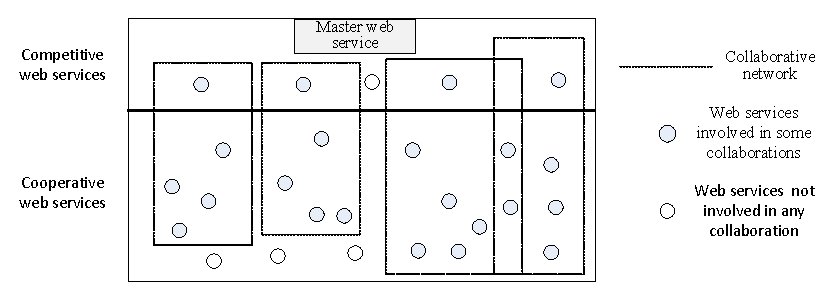
\includegraphics[scale=1]{architecture++.eps}
\caption{Web services are partitioned into competitive and
cooperative sets. Competitive web services may get tasks directly
from the master web service and they can share it with other
cooperative web services in their collaborative networks.}
\label{architectureFigure}
\end{figure}

\subsection{The Architecture}

The proposed system consists of three types of autonomous entities
with different goals.

1) \textit{Web Services} that reside inside a community which
aggregates a number of functionally similar or complementary web
services as a group (more details about communities of web
services are given in \cite{Khosravifar2010}). Within the same
community, each web service might have a network consisting of
some other web services that might get involved in a cooperative
work (e.g. composition and substitution). As web services are also
competing, particularly when they provide similar functionalities,
each one of them aims to maximize its individual income (i.e. the
payoff) by adopting a given strategy.

2) \textit{Master Web Service} is the manager and representative
of the community of web services. Among other functionalities, the
master web service is responsible for allocating the tasks to web
services within the community. After the task being accomplished,
the master rewards or penalizes the associated web service with
respect to its reputation as a member of the community. The master
is equipped with a task allocation mechanism aiming to increase
service users satisfaction and eventually the community's market
share in the whole system.

3) \textit{Users} generate tasks with specified QoS. In our
proposed system, tasks are continuously being generated and user
satisfaction is abstracted since we focus on web services'
interactive strategies.

Figure \ref{architectureFigure} illustrates the architecture of a
typical community aggregating a number of web services with
different interactive strategies. Some of them compete for the
task where they directly deal with the master. Some others
cooperate in the associated task where they only deal with the
competed web service as the task leader and do not directly
interact with the master (the master deals only with the web
service that has bid for the task, which is responsible of
choosing its collaborative network). In both sets, some web
services are for certain moments out of any collaboration network.
We highlight details of the interactive strategies in the rest of
this section.
%Figure \ref{algorithm1} %exposes the details of task allocation mechanism that is used to select the web services.
In the proposed system, the master sorts the competing web
services based on some parameters (such as reputation) that we
explain in the rest of this section. If the web service is busy or
unwilling to take the task, the master allocates the task to the
second competing web service in the list. There is a chance that
some tasks could not be assigned to any web service. These tasks
are accumulated to the task pool to be allocated in the next task
allocation round. Upon allocation of the task, the web service is
responsible to offer the required QoS that is stated in the task
being generated by a consumer. Afterwards,  the master rewards or
penalizes the competing web service by upgrading or degrading its
reputation according to the offered QoS compared with the required
one. This comparison influences the sorting mechanism used by the
master to allocate the tasks in further task allocation rounds.


%\begin{figure}[h]
%\centering
%\begin{tabular}{l}
% \hline\hline
%\textbf{Algorithm} Task Allocation Mechanism Used by Master Web Service\\  \hline
%  \small\textbf{CompetitiveWebServices}: Make a list of all web services ready to compete flag equal to %true\\
%  SortTaskPool(taskPool)\\
%  \small\textbf{TaskToBeDone}: Select a random number of undone tasks to be allocated\\
%  \small 1: \textbf{foreach} task \textbf{in} CompetitiveWebServices\\
%  \small 2: ~~~~~ \textbf{while} (!task.assigned)\\
%  \small 3: ~~~~~~~~~~~ \textbf{foreach} webservice \textbf{in} CompetitiveWebServices\\
%  \small 4: ~~~~~~~~~~~~~~~~~ \textbf{if}(!webservice.busy)\\
%  \small 5: ~~~~~~~~~~~~~~~~~~~~~~~ \textbf{if}(webservice.acceptTheTask)\\
%  \small 6: ~~~~~~~~~~~~~~~~~~~~~~~~~~~~~webservice.NumberOfOfferedTask+=1\\
%  \small 7: ~~~~~~~~~~~~~~~~~~~~~~~~~~~~~webservice.NumberOfAcceptedTask+=1\\
%  \small 8: ~~~~~~~~~~~~~~~~~~~~~~~~~~~~~webservice.CurrentAssignedTask=task\\
%  \small 9: ~~~~~~~~~~~~~~~~~~~~~~~~~~~~~task.assigned=true\\
%  \small 10: ~~~~~~~~~~~~~~~~~~~~~~~~~~~\textbf{break}\\
%  \small 11: ~~~~~~~~~~~~~~~~~~~~~~ \textbf{else}\\
%  \small 12: ~~~~~~~~~~~~~~~~~~~~~~~~~~~webservice.NumberOfOfferedTask+=1\\
%  \small 13: ~~~~~~~~~~~~~~~~~~~~~~~~~~~webservice.NumberOfRefusedTask+=1\\
%  \end{tabular}
%%
%\caption{Master web service task allocation algorithm that is used to allocate continuous tasks to %appropriate competitive web services.} \label{algorithm1}
%\end{figure}



\subsection{System Parameters}
In this part, we demonstrate the involved parameters and their
corresponding formulations and explanations.

\textbf{Task QoS} ($T_{QoS}^t$) is the required QoS metric for a
specific task at time $t$. Users define tasks with specific QoS
requirements such as response time, availability, and
successability (or accuracy) \cite{Erbin}. We aggregate and
normalize these metrics to a value between $0$
and $1$. %Throughout this paper, we refer to this value as
%$T_{QoS}$.

\textbf{Web service QoS} ($QoS_w^t$) is the QoS provided by the
web service $w$ after performing a task at time $t$. Again the
metrics that contribute in computing this QoS are aggregated and
normalized to a value between $0$ and $1$. The offered quality
might or might not meet the required task quality $T_{QoS}^t$. In
the latter case, the service user would be disappointed and a
negative satisfaction feedback is expected. In our proposed
system, both cases are considered when calculating the web
services' reputation.

%\textbf{NTD} is the number of tasks completed by a web service.

\textbf{Budget} ($B_w^t$) is the amount of money the web service
$w$ has in its disposal at time $t$, which helps pay for the
community membership fees ($\epsilon$) and is one of the
parameters that the web service considers when deciding about
getting involved in a competition or not. This parameter has been
used in other service computing settings such as \cite{Erbin}.

\textbf{Reputation} is a factor in any online community where
trust is important. Without any trust enabling mechanism, users
cannot differentiate between services, specially the ones which
offer the same type of service. Reputation mechanisms usually
aggregate users' experiences and in our case it strongly depends
on QoS that each web service provides. Users define tasks with
specific quality $T_{QoS}^t$, therefore after performing a task
with $QoS_w^t$, the reputation of $w$ gets evaluated by the master
web service. $Rep_{w}^{t}$ refers to the reputation of $w$ at time
$t$.

In Equation \ref{repr}, we compute the reward that the master
computes considering the task QoS compared with the web service
offered quality $QoS_w^t$. In case the offered quality meets user
expectations, the reward value would be positive. In this system,
we consider a small value as default rewards $\eta$ which the
master considers together with the proportional level of
satisfaction as a weighted value (by $\upsilon$). In this case,
the higher the offered quality is, the more weighted reward is. In
case the offered quality did not meet the user expectations, the
reward would be negative. In this case, we also have a default
penalty value $\rho$ (where $\rho>\eta$) together with the
weighted proportional difference. The idea is to harshly penalize
the web services rather than rewarding them. To this end, rational
web services should carefully analyze their capabilities once the
available tasks are announced. In our proposal, web services have
the goal of increasing their budget, which is directly related to
their reputation. Thus, they have to decide strategically how to
maximize this value.

\begin{equation} \label{repr}
reward_w^t= \begin{cases}
\eta + \frac{QoS_w^t}{T_{QoS}^t+QoS_w^t} * \upsilon  & \text{if $T_{QoS}^t\leq QoS_w^t$;}\\
-(\rho + \frac{T_{QoS}^t}{T_{QoS}^t+QoS_w^t} * \upsilon) & \text{otherwise.}\\
\end{cases}
\end{equation}

The assigned reputation value is updated by the computed reward
value. The computed reputation of web services is bounded by the
minimum and maximum reputation values $0$ and $1$. % to constrain
%the balance the cooperative community of web services. The updated
Let $\Gamma = Rep_{w}^{t} + reward_w^t$. The updated reputation
value is then computed as follows:

\begin{equation}\label{repz}
%Rep_{w}^{t+1} = Rep_{w}^{t} + reward
%\end{equation}
%\begin{equation*}
Rep_{w}^{t+1} = \begin{cases}

\Gamma & \text{if $ 0 \leq \Gamma \leq 1$;}\\
0  & \text{if $\Gamma < 0$;}\\
1 & \text{if $\Gamma > 1$.}\\
\end{cases}
\end{equation}

\textbf{Growth Factor} is a parameter which declares web services'
performance based on their recent strategies and activities.
Growth factor is relative to web services' reputation and QoS.
This parameter is the main variable a typical web service uses to
decide which strategy to adopt. The details about the decision
making process is described in Section \ref{Theoretical Results}.
We use Equation \ref{eq:growthfactor} to compute the growth factor
$G^t_w$ of the web service $w$ at time $t$. The growth factor
function should be monotonically increasing in $QoS_w^t$,
$Rep^t_w$ and $B_w^t$, which is satisfied by the equation and this
could be easily proven by calculating the partial derivatives of
this function in 1) $QoS_w^t$; 2) $Rep^t_w$; and then 3) $B_w^t$
and show that they are all positive. The contribution of the
budget $B_w^t$ in the calculation of the growth factor should be
proportional to the ideal budget $\beta_w \times t$ where the web
service receives all the offered tasks during the periods $t$. The
parameter $\beta_w$ denotes the profit obtained considering the
mean received service fee $\mu_w$ and the cost of community
membership $\epsilon$. The mean service fee depends on the
strategy adopted by the web service because a competitive service
receives higher fees $\mu_{w, CM}$ compared to a cooperative one
$\mu_{w, CO}$ ($\mu_{w, CM} > \mu_{w, CO}$). The motivation behind
this is that a competitive web service for a given task is the
leader for that task while other cooperative web services are
performing specific subtasks as asked by the leader.


\begin{equation}\label{eq:growthfactor}
G^t_w = \frac{Rep^t_w + QoS_w^t+\frac{B_w^t}{t\times \beta_w}}{3}
\end{equation}
\begin{equation*}
\beta_w=\mu_{w}-\epsilon, ~~~~~~\mu_{w} \in\{\mu_{w, CM}, \mu_{w,
CO}\}
\end{equation*}

The above explained parameters and other additional parametrs
which we will use in the rest of this paper are listed in Table
\ref{Preliminaries}.


\begin{table}
\centering
\caption{List of proposed system parameters.}
\begin{tabular}{|c|c||c|c|}
\hline
\textbf{Notation} & \textbf{Definition} & \textbf{Notation} & \textbf{Definition}\\
\hline\hline
$T_{QoS}^t$ & Required task QoS at time $t$ & $QoS_w^t$ & Web service $w$ QoS at time $t$ \\
$B_w^t$ & Budget associated to web service $w$ at time $t$ & $Rep^t_w$ & Reputation assigned for $w$ at time $t$\\
$Reward_w^t$ & The reward to update the reputation & $G^t_w$ & The growth factor of $w$ at time $t$\\
$\epsilon$ & The community membership fee & $\pi_{w,CM}^t$ & Competition payoff of $w$ \\
$\pi_{w,CO}^t$ & Cooperation payoff of $w$ & $p_{w,CM}^t$ & Competition probability of $w$ at time $t$\\
$p_{w,CO}^t$ & Cooperation probability of $w$ at time $t$& $COF_w^t$ & Cooperation fee of $w$ at time $t$\\
$\beta_w$ & Profit of $w$& $\mu_{w, CM}$ & Mean service fee for competing $w$ \\
$\mu_{w, CO}$ & Mean service fee for cooperating $w$ & $\tau_w^t$ & Coopetitive threshold of $w$ at time $t$ \\
$P_w^t$ & Probability of competing for $w$ at time $t$& $U_w^t$ & Utility of $w$ at time $t$\\
\hline
\end{tabular}
\label{Preliminaries}
\end{table}

\subsection{Web Service Interactive Strategies}

The main goal of each individual web service is to increase its
income (payoff). This income can be earned from tasks (or
requests) done by this web service. In our model, web services can
decide to compete to get a task from the master web service or to
cooperate with other web services in a given collaborative network
(the way a collaborative network is set by a leader is based on
the cooperative web services reputation and their QoS parameters
that should coincide with the required QoS). Therefore we define
two types of web service strategies; when a web service has higher
level of confidence based on its growth factor, it can compete to
get a task from the master and adopts the competitive strategy. On
the other hand, when it has a lower level of confidence that it
does not feel it can compete with other web services to get a
task, the web service waits for some other web services to
cooperate with for completing a task and thus it adopts the
cooperative strategy. Web services estimate the outcome of all the
strategies and choose one of them accordingly. This decision is
not static but can change over time so web services can switch
from one strategy to the other and this dynamic attitude is
referred to as coopetition. We discuss about this decision making
process in more details in the next section.








\section{Theoretical Results}\label{Theoretical Results}

\subsection{Web Service Decision Making Procedure}
%In the previous section, we introduced web services' interaction
%strategies.
In this section, we explore in details the interaction strategies
and the outcome of each strategy in terms of web services'
utilities. The main part of web services' decision making
procedure falls into their growth factor analysis. In fact, the
growth factor and its comparison to a particular threshold is the
main reason that influences the web service's decision to follow
either competitive or cooperative behavior. Web services initially
compute this value and compare it with their computed threshold.
Generally the main challenge is the threshold computation and we
cope with this issue in the rest of this section. We additionally
use the obtained results in the implemented environment and
analyze their effectiveness on web services' strategic decision
making procedures.


Figure \ref{decisionMakingProcedure} shows the decision making
process that is followed by a typical web service. In case the web
service is ready to compete, there is a chance that it bids for a
task if it has the required capabilities to accomplish that task,
or stays silent and returns to the cooperative status. But in case
the web service is willing to cooperate, it has to wait for a
cooperation opportunity that could be triggered by another web
service that competed and obtained the task, so both web services
will be part of the same collaborative network. In the decision
making process presented in Figure \ref{decisionMakingProcedure},
we assume that the competing web service might get the task
(denoted as $Bid/obtainedTask$) or not get the task in case of
being rejected by the master web service, or do not even bid for
the task (denoted as $Silent/rejectedTask$). For simplicity
reasons and without loss of generality, we group the two cases of
$Bids$ and $obtainedTask$ together as well as $Silent$ and
$rejectedTask$. The rational behind this aggregation is the fact
that our main concentration is web services' status (competitive
or cooperative) over different decision making rounds which could
be caused by internal factors (the web services) or by the
external factor (the master web service).

\begin{figure}[h]
\centering
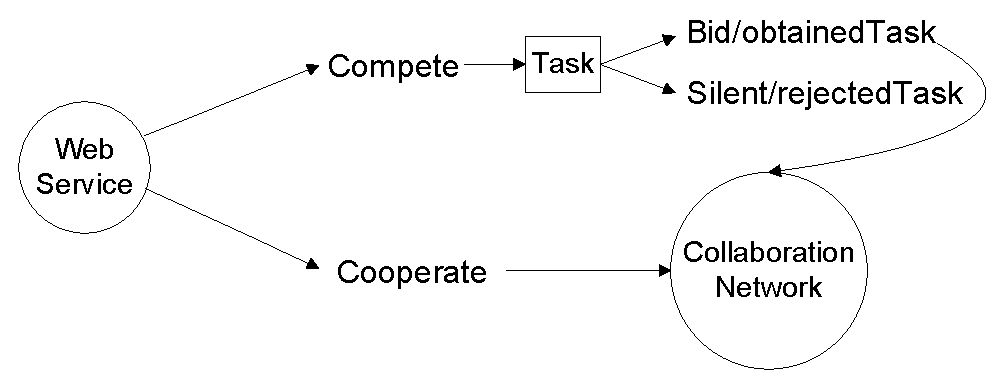
\includegraphics[scale=0.45]{decision1++.eps}
\caption{Decision making process over competitive and cooperative
strategies.} \label{decisionMakingProcedure}
\end{figure}





Consider a web service $w$ that is willing to compete (that means
the computed growth factor is more than the analyzed threshold).
This web service can estimate the expected payoff associated to
this decision, called competition payoff. Equation \ref{CMPff}
computes this expected payoff for web service $w$ ($\pi_{w,CM}^t$)
considering the $Bid/obtainedTask$ probability of $p_{w,CM}^t$ and
$Silent/rejectedTask$ probability of $1-p_{w,CM}^t$.

\begin{equation}\label{CMPff}
\pi_{w,CM}^t=p_{w,CM}^t(\mu_{w,
CM}-COF_w^t-\epsilon)+(1-p_{w,CM}^t)(-\epsilon)
\end{equation}

In Equation \ref{CMPff}, $\mu_{w, CM}$ is the mean service fee
that is assigned by the master web service to $w$. This means that
a competing web service $w$ directly obtains this fee from the
master web service. Moreover, the competing web service $w$
expects a cooperation fee ($COF_w^t$) that it gives to its
collaborators in case $w$ needs to cooperate with other web
services (cooperative web services in its collaboration network).
In any case, the competing or cooperating web service pays a fixed
amount of membership ($\epsilon$) to the master web service as the
coordinator of the community. This fee would be taken into account
when a web service decides to leave to a cheaper community or act
alone. But to concentrate on the main concerns of this paper, we
skip these small details.


Similar to the competitive web service case, if a web service $w$
declares cooperative status, its expected cooperation payoff
($\pi_{w,CO}^t$) is computed in Equation \ref{CLPff}. In this
equation, $p_{w,CO}^t$ is the probability of getting involved in a
cooperative task with other web services and $1-p_{w,CO}^t$ is the
probability of failure to find such a cooperation opportunity.
These two probabilities are set when $w$ decides to compete. We
recall that $\mu_{w, CO}$ denotes the mean cooperation fee that is
directly obtained from the leader (i.e., the competitive) web
service of the underlying collaborative network. Compared to
$\mu_{w, CM}$, $\mu_{w, CO}$ is relatively smaller since the
competitive web service generally dedicates a portion of its
obtained income to pay other cooperative web services.


\begin{equation}\label{CLPff}
\pi_{w,CO}^t=p_{w,CO}^t (\mu_{w,
CO}-\epsilon)+(1-p_{w,CO}^t)(-\epsilon)
\end{equation}


To analyze the expected payoffs obtained from different
strategies, web services need to compute the estimated
probabilities that distinguish subcases in each behaviorial status
($p_{w,CM}^t$ for competitive and $p_{w,CO}^t$ for cooperative).
To estimate these probabilities, we should notice that they are
functions of web services' reputation values ($Rep_w^t$).
Furthermore, $p_{w,CM}^t$ is also function of the difference
between the offered QoS ($QoS_w^t$) and the requested one
($T_{QoS}^t$); and $p_{w,CO}^t$ is function of the reputation of
other web services in the community because the leader is supposed
to be selective when it comes time to choose the collaborators. To
this end, we first discuss the desirable properties of an
estimation function of each of these probabilities, and show that
the proposed ones satisfy those properties. The desired properties
of $p_{w,CM}^t$ are as follows:

\begin{property}
$p_{w,CM}^t$ is continuous with regard to $Rep^t_w$, $QoS_w^t$,
and $T_{QoS}^t$.
\end{property}
%
\begin{property}
$p_{w,CM}^t$  is monotonically increasing/decreasing in $Rep^t_w$
and $QoS_w^t - T_{QoS}^t$ while $QoS_w^t - T_{QoS}^t$ is positive.
\end{property}
%
\begin{property}
$p_{w,CM}^t$ is null if $QoS_w^t - T_{QoS}^t$ is negative.
\end{property}
%
%\begin{property}
%Assuming that the web service $w$ is known by the master web
%service, $Rep^t_w$ is monotonically increasing or decreasing in
%$QoS_w$.
%\end{property}
%
\begin{property}
The increase slope of $p_{w,CM}^t$ is higher when the reputation
$Rep^t_w$ increases in the interval $[0, 0.5]$ than when it
increases in the interval $]0.5, 1]$.
\end{property}


\noindent Property 1 simply says that the probability of success
competition $p_{w,CM}^t$ can be always estimated as far as
$Rep^t_w$, $QoS_w^t$, and $T_{QoS}^t$ are available. Property 2
says that the reputation and QoS are two key factors that
influence the value of $p_{w,CM}^t$ in the sense of positive
correlation. Property 3 indicates that the probability
$p_{w,CM}^t$ is null if the offered QoS is less than the
expectation. Property 4 promotes the increase of the reputation
for new comers and imposes higher increase rate at the beginning
of the reputation curve because it is always hard to build the
reputation, but once it is built, its maintenance is less
challenging.


\noindent The desired properties of $p_{w,CO}^t$ are as follows:

\begin{property}
$p_{w,CO}^t$ is continuous with regard to $Rep^t_w$ and the
reputation of other web services in the community.
\end{property}
%
\begin{property}
$p_{w,CO}^t$  is monotonically increasing in $Rep^t_w$ and
 monotonically decreasing in the community average reputation.
\end{property}
%
%\begin{property}
%$p_{w,CM}$ is null if $QoS_w^t - T_{QoS}^t$ is negative.
%\end{property}
%
%\begin{property}
%Assuming that the web service $w$ is known by the master web
%service, $Rep^t_w$ is monotonically increasing or decreasing in
%$QoS_w$.
%\end{property}
%
\begin{property}
The increase slope of $p_{w,CO}^t$ is higher when the reputation
$Rep^t_w$ increases in the interval $[0, 0.5]$ than when it
increases in the interval $]0.5, 1]$.
\end{property}

\noindent Property 5 is similar to Property 1. Property 6 says
that $w$ has more chance to get involved in a cooperation if it
has high reputation compared to the other members. This chance
decreases if other web services have higher reputation. Property 7
is similar to Property 4.

Equations  \ref{CMp_w} and \ref{CLp_w} respectively compute the
estimated success probability in cases where the web service $w$
is competing and cooperating. These values are computed
considering web service's reputation value ($Rep^t_w$ computed by
the master), web service's offered QoS ($QoS_w$), the task
required QoS ($T_{QoS}^t$) which is the mean required QoS computed
from previous tasks, the maximum offered QoS ($QoS_k^t$, which is
provided by another competitive web service $k$), and the
cooperative factor $CL_w^t$ of the web service $w$ at time $t$,
which is computed as the portion of web service's current
reputation on the average reputation of the community.

\begin{equation} \label{CMp_w}
p_{w,CM}^t = \begin{cases}
\sin(Rep^t_w\frac{\pi}{2})\frac{QoS_w^t-T_{QoS}^t}{Max_k(Qos_k^t-T_{QoS}^T)} & \text{if $QoS_w^t\geq T_{QoS}^t$;}\\
0 & \text{otherwise.}\\
\end{cases}
\end{equation}

\begin{equation}\label{CLp_w}
p_{w,CO}^t=sin(Rep^t_w\frac{\pi}{2})CL_w^t
\end{equation}
\begin{equation*}
CL_w^t=\frac{Rep^t_w}{\sum_{k\in Community}Rep^t_k/|Community|}
\end{equation*}



It is easy to prove that Equation  \ref{CMp_w} satisfies Property
1. The partial derivative $\frac{\partial p_{w,CM}^t}{\partial
Rep^t_w}$ is positive as the function $\cos$ (the derivative of
$\sin$) is positive on $[0, \frac{\pi}{2}]$ and $Rep^t_w \in [0,
1]$. The partial derivative $\partial p_{w,CM}^t$ with regard to
$QoS_w^t - T_{QoS}^t$ is also positive, which proves the
satisfaction of Property 2. Property 3 is straightforward.
Finally, the increase slope of the function $\sin$ on $[0,
\frac{\pi}{2}]$ proves Property 4.

Similarly, we can easily prove that Equation \ref{CLp_w} satisfies
Property 5. Property 6 can be shown by calculating the partial
derivative $\partial p_{w,CO}^t$ first with regard to $Rep^t_w$
and second with regard to the community average reputation
$\sum_{k\in Community}Rep^t_k/|Community|$. The first partial
derivative is positive and the second is negative, which proves
the satisfaction of Property 6. The proof of satisfaction of
Property 7 is similar to the one of Property 4.

%Considering these involved parameters, we verify that properties
%$1$ to $3$ are satisfied. For property $4$, we use $sinus$
%function to promote the role of reputation influence in this
%system. Using $sinus$ function, we promotoe reputation increase of
%web sevrices specially when it is less than $50\%$. Considering
%the desired properties, the formulas represented in Equations
%\ref{CMp_w} and \ref{CLp_w} are candidates we chose to compute the
%probabilities regarding $Competitive$ and $Cooperative$
%strategies. These formulas are used in implemented system and
%verified with respect to their accuracy and effectiveness in
%adopting different interacting strategies.


%In the proposed heuristic  function, the web service $w$ is not
%aware of current $T_{QoS}$ and $QoS_k$, but could use its previous
%information to estimate their values. To this end, if the web
%service is more informative about the previous data, it could
%obtain more realistic measurement over the estimated
%probabilities.
%
%
%We compute the success probability of cooperation ($p_{w,CO}$)
%similarly in the sense  that we still promote reputation influence
%using $sinus$ function, but multiplied to the cooperative factor
%$CL_w$ of the web service $w$. This value is computed as the
%portion of web service's current reputation on the average
%reputation of the community.


\subsection{Coopetition Threshold}

In this part, we compute the coopetition threshold that a typical
web service could use to adopt reasonable interacting strategies
and we empirically verify the effectiveness of the obtained
results in the next section. In fact, to decide which strategy to
adopt, we let the web service $w$ compare its growth factor
($G_w^t$) with the coopetition threshold it holds at current time
$t$ ($\tau_w^t$) and choose to compete with probability $P_w^t$
that we compute in Equation \ref{P}. Based on this probability, we
calculate the total utility $U_w^t$ in Equation \ref{U}.

\begin{equation} \label{P}
P_w^t= \begin{cases}
\frac{G_w^t}{\tau_w^t}  & \text{if $G_w^t\leq \tau_w^t$;}\\
1 & \text{otherwise.}\\
\end{cases}
\end{equation}

\begin{equation}\label{U}
U_w^t=P_w^t(\pi_{w,CM}^t)+(1-P_w^t)(\pi_{w,CO}^t)
\end{equation}


%Equation  \ref{U} computes the
%expected utility (as accumulated fee) regarding web service $w$.
%This estimated utility is result of aggregation of two different
%interacting strategies of $Competitive$ and $Cooperative$.
%Aggregating these strategic payoffs, web service $w$ follows
%probability distribution of $\{P,1-P\}$. This probability
%distribution is computed in Equation \ref{P}, which is a function
%of the growth factor ($G_w$) and computed threshold ($Tr^t$). So
%if the web service is aware of the reasonable threshold, the value
%$p$ could be computed and used as the core of strategic
%probability distribution. But there is a case where the web
%service does not have a reasonable threshold value and cannot
%rigorously decide for any adopting strategies.


The key factor in the computation of the probability $P_w^t$ and
the associated utility is the threshold value. To compute the
threshold, we use the game theoretic best response technique. A
typical web service $w$ will follow the best response strategy to
maximize its expected aggregated payoff. The idea is to equalize
the expected payoffs of the two acting strategies: compete and
cooperate.
%
%
%by following the following three probability distributions: (1)
%$\{1,0\}$ where the web service always competes; (2) $\{0,1\}$
%where the web service always cooperates; and (3)
%$\{\frac{1}{2},\frac{1}{2}\}$ where the web service equalize the
%probabilities and decides with unbiased distribution. Following
%the third case, the web service equits the expected payoffs as
%outcomes of different interacting strategies.
%
The objective behind equalizing payoffs is to explore conditions
under which the web service $w$ could react with best response to
further decision making procedures. We use the obtained conditions
to compute the threshold $\tau_w^t$ at time $t$. By equalizing
$\pi_{w,CM}^t$ and $\pi_{w,CO}^t$, we obtain:

\begin{equation*}\label{equit}
\pi_{w,CM}^t=\pi_{w,CO}^t      \rightarrow
\end{equation*}
\begin{equation*}
p_{w,CM}^t(\mu_{w,CM}-COF_w^t-\epsilon)+(1-p_{w,CM}^t)(-\epsilon)=p_{w,CO}^t(\mu_{w,
CO}-\epsilon)+(1-p_{w,CO}^t)(-\epsilon)
\end{equation*}
The fixed membership fee $\epsilon$ could be taken out and
canceled from both sides of the equation so we obtain the
following:
\begin{equation*}
p_{w,CM}^t(\mu_{w,CM}-COF_w^t)=p_{w,CO}^t(\mu_{w,CO})\rightarrow
\end{equation*}
\begin{equation*}
sin(Rep^t_w\frac{\pi}{2})\frac{QoS_w^t-T_{QoS}^t}{Max_k(Qos_k-T_{QoS}^t)}(\mu_{w,
CM}-COF_w^t)=sin(Rep^t_w\frac{\pi}{2})CL_w^t(\mu_{w, CO})
\end{equation*}
By simplifying the $sinus$ variable from both sides and
substituting the cooperation factor $CL_w^t$ of the web service
$w$ we obtain the following:
\begin{equation*}
\frac{QoS_w^t-T_{QoS}^t}{Max_k(Qos_k^t-T_{QoS}^t)}(\mu_{w,CM}-COF_w^t)=\frac{Rep^t_w}{\sum_{k\in
Community}Rep^t_k}(\mu_{w, CO})
\end{equation*}
%
We use the obtained equation to obtain the cooperation fee
$COF_w^t$ that is assigned by the web service $w$. This fee
represents the amount that $w$ spends to cooperate with other web
service(s) to accomplish the task. By so doing, we obtain the
maximum amount of cooperation fee that the web service $w$ can use
to constrain the positive payoff out of competing. Otherwise, the
web service stays as cooperative entity. The cooperation fee is
computed in Equation \ref{CLF}.

\begin{equation}\label{CLF}
COF_w^t=\mu_{w,CM}-\frac{Rep^t_w}{\sum_{k\in
Community}Rep^t_k}\frac{\mu_{w,CO}Max_k(Qos_k^t-T_{QoS}^t)}{QoS_w^t-T_{QoS}^t}
\end{equation}

We use the maximum cooperation fee that a web service considers to
constrain the positive expected payoff when the competitive
strategy is adopted to update the threshold for the consequent
time interval ($t+1$). We compare the maximum cooperation fee with
the required fee ($ReqF_w^t$) that the web service indicate to
accomplish the task. The outcome of this comparison is a factor
that uses the current threshold $\tau_w^t$ to compute the
consequent threshold $\tau_w^{t+1}$. As in online learning, the
idea is to compute iteratively the threshold until the fixed point
is achieved, which indicates the threshold's conversion, where the
initial value is randomly chosen (in the simulation different
initial values are used). Equation
\ref{Trt} shows this computation. %We restrict the range of this value to $(0.15,0.85)$ to
%avoid some unreasonable results that could occur due to different
%reasons like system start point or heavy loaded competitive web
%services, \textit{etc}.
To investigate the effectiveness of this threshold on the outcomes
of the web services that follow this reasoning technique, in the
next section, we compare the results of different agents with
diverse strategic reasoning techniques.

\begin{equation}\label{Trt}
\tau_w^{t+1}=\begin{cases}
\Theta & \text{if $0 \leq \Theta \leq 1$}\\
1 & \text{if $\Theta > 1$;}\\
0 & \text{if $\Theta < 0$.}\\
\end{cases}
\end{equation}
\begin{equation*}
\Theta =\tau_w^t \times \frac{COF_w^t}{ReqF_w^t}
\end{equation*}



\section{Experimental Results}\label{Experimental Results}

In this section, we provide an empirical analysis over the
observed results regarding the characteristics of intelligent web
services hosted in different communities of web services. In the
implemented system, we simulate the behaviors of service consumers
as request generators, web services as service providers, and
master web services as community representatives. These entities
are developed with respect to what is explained in Section
\ref{Preliminaries}. The objective is to investigate the
effectiveness of the proposed strategic system on intelligent
web services' overall budge and also the average QoS of tasks performed by 
community web services which directly affects user satisfaction. 
%Before conducting the simulation, the
%expected behavior of our model is to enhance the budget of web
%services when using our proposed strategic interacting system.
%Although this result is promising, we would like to investigate
%the effectiveness of the proposed strategic system on intelligent
%web services' overall budget compared to the best case. Moreover,
We study the overall performance of the community hosting the
reasoning-empowered web services compared to the ones hosting
stochastic and purely competitive services. The simulation
application is written in \textit{C\#} using \textit{Visual Studio}. 
Developed web services are initialized with values taken
from a real dataset that includes $2507$ real web services
functioning on the web. The dataset records the QoS values of $9$
parameters including \textit{availability}, \textit{throughput},
and
\textit{reliability} \cite{Almasri}.  %These QoS values
%are determined by monitoring the web services over a $6$-day
%period.





We start our discussions with cumulative budget comparison
regarding different communities within which services follow
different reasoning techniques. Figure \ref{Graph1} part (a)
illustrates three graphs for three different communities. Each
community hosts web services that follow different reasoning
techniques: (1) a community that follows the interactive reasoning
techniques presented in this paper (referred to as coopetitive);
(2) a community that follows a random reasoning technique so
decisions about selecting competitive or cooperative strategies
are totally random (referred to as random coopetitive); and (3) a
competitive community where all services follow the competitive
strategy (referred to as competitive). The proposed model's
reasoning mechanism enables services to effectively select their
interacting strategies and the obtained budget represents the best
outcome over the strategic decision making procedure they run all
the time. This procedure avoids cases where a service selects the
competitive strategy but gets refused to obtain a task from the
master. The procedure allows services to make decisions that
maximize their utilities, so that if the web service cannot
compete, the procedure would suggest to collaborate, which is
better than competing and failing to obtain the task. In this case
(i.e., competing and not getting the task), the service stays idle
but still pays the community membership fee, which means losing
utility. The developed strategic decision making mechanism leads
some web services to follow cooperative strategies that overall
maintain an optimal community budget. In the same figure, we
observe the cumulative budget of a community where services follow
random interacting strategies. The outcome is clearly lower
because services at each run randomly decide over their acting
strategies. This potentially influences the community budget
because a low quality service if randomly selects to follow the
competitive strategy, it will fail to perform a task with high QoS requirements. This kind of
strategy selection is totally stochastic while the task allocation
algorithm follows a logical path. The ideal system is the one that
analyzes the optimal strategic path and consistently follows
strategies that bring maximum outcome. The result regarding the
community that follows the random strategy shows how stochastic
decision making degrades the community budget, but still this
result outperforms the one of the purely competitive community. In
the last case, all the services follow the competitive strategy
and the frequency of getting rejected from a task is relatively
high. In a community with limited number of tasks, the competitive
strategy for all services highly influences the community budget
because a potential group of services are losing at every run.

\begin{figure}%[h]
\centering
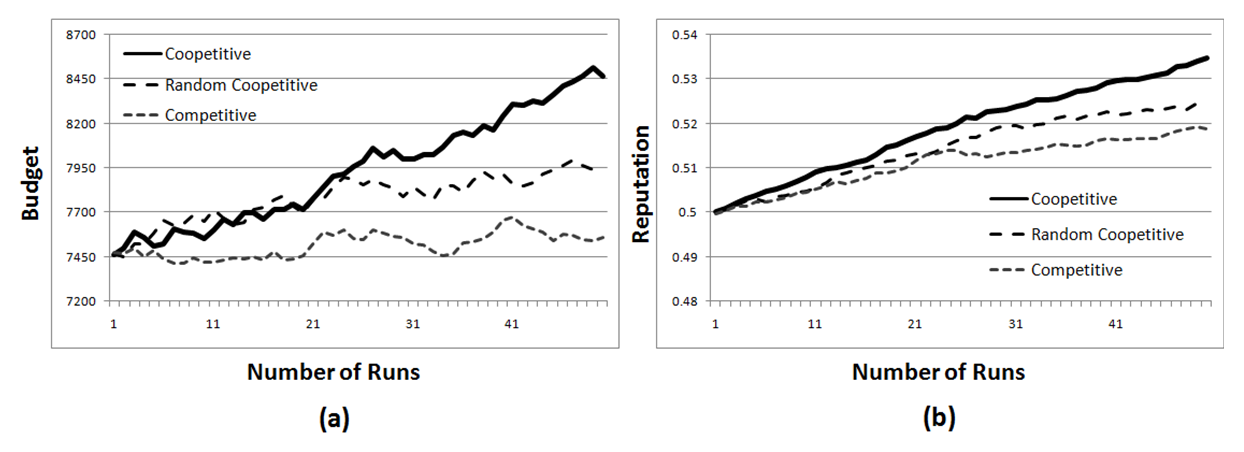
\includegraphics[scale=0.6]{graph1Final+.eps}
\caption{Part (a): Cumulative community budget comparison. Part
(b): Average community reputation comparison over different
strategic decisions.} \label{Graph1}
\end{figure}




The results illustrated in Figure \ref{Graph1} part (a)  verify
the importance of the strategic decision making procedure to
logically decide over the possible competitive and cooperative
choices. Figure \ref{Graph1} part (b) illustrates communities
average reputation of involved web services. The graphs represent
the influence of the rewards that the master web service imposes
to encourage highly capable web services to compete for a task. As
for the cumulative budget, we observe that the coopetitive
community outperforms the random coopetitive and competitive
communities in terms of average reputation. The proposed model's
average reputation increases because web services follow optimal
strategies where they can perform better so obtain higher rewards.
For the same reasons as for the cumulative budget, the average
reputation of the random coopetitive community
outperforms the one for the coopetitive community. %The idea is to balance web
%services' strategies to maintain optimal community budget.


 %Figure \ref{Graph2} part (a) illustrates the reputation of the proposed $Coopetitive$ community where
 %we highlight the range of reputation change in the community. The vertical lines denote the range of %reputation that is associated with the master web service. The rewards and penalties applied to %different
% web services show that the master web service over runs extends the reputation range and takes %control of the whole community. In the developed model, web services are encouraged to choose
 %optimal staretgies. This is maintained over growth factor comparison of the $Coopetitive$ web %sevrvices.

Figure \ref{membership_fee_graph} depicts how increasing the membership fee which is analogious to getting lower amount of income when doing tasks successfuly affects the overall budget of webservices using different decision making processes. In Figure \ref{membership_fee_graph} part(a) we set the membership fee to 2, in \ref{membership_fee_graph} part(b) to reletively high value of 5 and \ref{membership_fee_graph} part(a) shows the result when the membership fee is set to very high fee of 10. 


In Figure \ref{Graph2} parts (a) and (b), we observe the
competitive and cooperative probability of four different web
services where two of them ($w_1$ and $w_3$) are following optimal
strategies (competitive for $w_1$ and cooperative for $w_3$) and
the two others ($w_2$ and $w_4$) are following non-optimal
strategies. Over elapsing runs, web services that follow optimal
strategies bring best budget. In fact, the master web service
rewards the high quality web service that chooses the competitive
strategy, cooperates with other web services and successfully
accomplishes the task. In this system, the reputation regarding
such a web service is increasing over time and the possibility of
allocating further tasks is increasing as well. By increasing the
growth factor, such a web service (here shown as $w_1$) increases
the probability of selecting the competitive strategy. On the
other hand, the other web service (here shown as $w_2$) that is
incapable of competing is penalized by the master web service
because the offered quality might not meet the required task
quality. Thus, $w_2$ degrades its growth factor by following the
competitive strategy. As intelligent entity, this web service is
encouraged to change its strategy to the cooperative one and thus,
its probability of selecting the competitive strategy is
decreasing over time. We have similar results in Figure
\ref{Graph2} part (b) regarding web services $w_3$ and $w_4$ where
unlike $w_4$, $w_3$ is strategically following the cooperative
strategy. Therefore, $w_4$ is more seeking the competitive
strategy where it can increase its growth factor.

\begin{figure}%[h]
\centering
\includegraphics[scale=0.33]{Graphtest.eps}
\includegraphics[scale=0.33]{Graphtest.eps}
\caption{Competitive and cooperative probabilities regarding four
different web services.} \label{Graph2}
\end{figure}


We conclude our analysis by discussing the percentage of correct
strategy selection (Figure \ref{Graph3}). By this we mean the
average of web services that can get a task when the coopetitive
strategy is followed. We observe that in different runs, this
percentage is generally increasing. This shows that over runs the
web services get to learn the threshold $\tau_w^t$ that allows
them to select the good strategy. We should notice that in
different runs different initial values of the threshold are used
ranging from $0.3$ for run 1 to $0.6$ for run 4.

\begin{figure}%[h]
\centering
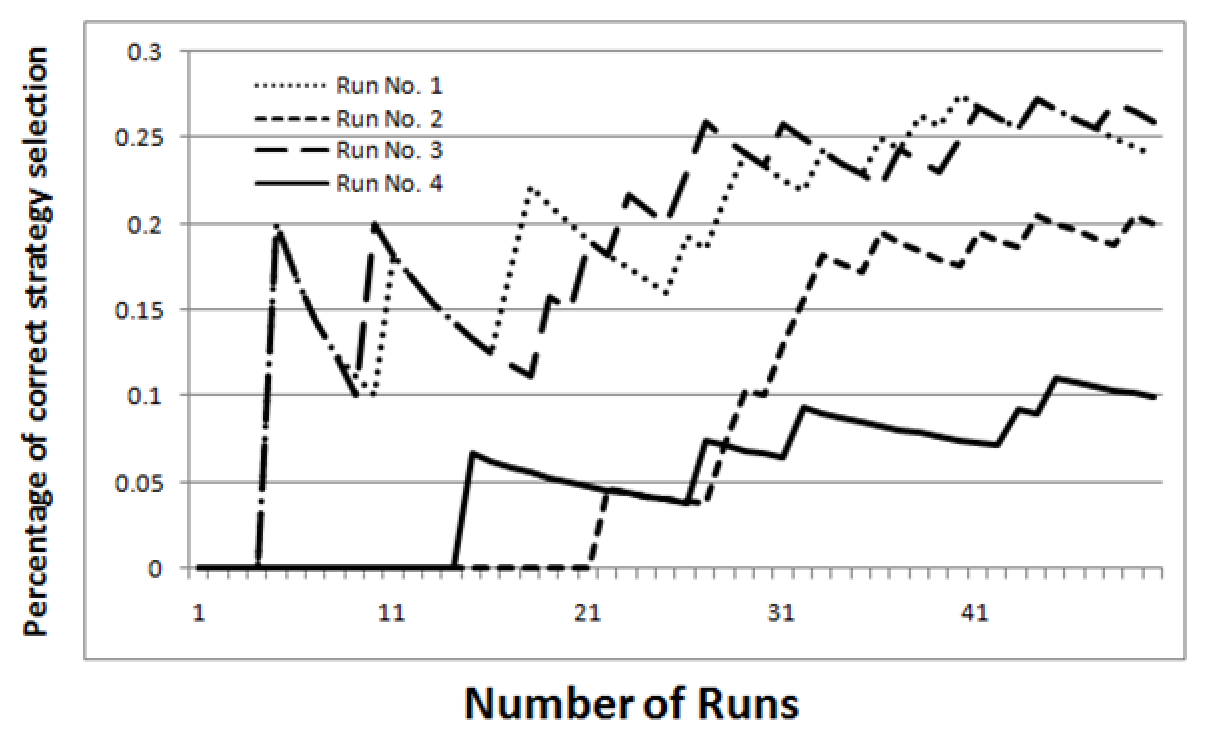
\includegraphics[scale=0.33]{graph3Final+.eps}
\caption{Percentage of correct strategy selection in different
runs using different initial threshold values.} \label{Graph3}
\end{figure}


%We conclude our analysis by discussion over the plots in Figure
%\ref{Graph3}. In this Figure, there are 6 plots that vertically
%refer to a scenario where we change some initialized settings. The
%upper plots represent the percentage of the correct strategy
%selections where is increasing in all scenarios but with different
%slopes. The lower plots illustrate the instant threshold together
%with the instant growth factor of a particular web service that
%follows the coopetitive strategy.

\section{Related Work and Conclusion}\label{Conclusion}

Relevant proposals to the model presented in this paper are the
ones that address service selection and task allocation
mechanisms. In many frameworks proposed in the literature, service
selection and task allocation are regulated based on the
reputation parameter \cite{Maximilien2,Kalepu,Rosario,Ruth}. In
\cite{Huang}, the authors propose a framework to match potential
benefits of web services while cooperating with one another. The
interesting idea is to consider the benefits under four
categories: innovation and learning, internal business process,
customer, and financial benefits. In \cite{Alchieri}, the authors
present a dependable framework for cooperative web services that
is based on the tuple space coordination model. The
intrusion-tolerant perspective is emphasized in this paper where
several security mechanisms are developed to enable a reliable
coordination system. %In \cite{Maximilien2}, authors propose
%ontology for quality of service. Users compute the web services'
%reputation using ratings.
The proposed frameworks mostly aim to facilitate the coordination
mechanism between web services. However, the opposite strategy of
competing is not analyzed where web services might be more
successful when competing within a same group. In fact, web
services are not always willing to cooperate even if they have
some common goals, particularly when they operate within groups
such as communities. In such a context, web services can follow
different interacting strategies and have to decide when to
compete and when to cooperate so that their ultimate goal,
maximizing their incomes, can be better achieved.

The contribution of this paper is the proposition of a coopetitive
strategic model to analyze the interacting behavior of intelligent
web services that are active within communities. We considered two
acting strategies where web services expect different sort of
payoffs: (1) competitive strategy where the web service claims
that it can accomplish a task, and therefore can take the
responsibility over the service consumer satisfaction; and (2)
cooperative strategy where the web service does not take the
responsibility to accomplish the task and only cooperates with
other competitive web services. Our proposed model advances the
state-of-the-art in cooperative systems by enabling intelligent
web services to effectively choose their interacting strategies
that lead to optimal outcomes. The proposed framework provides a
reasoning technique that web services can use to increase their
overall obtained utilities. The theoretical results presented in
this paper are also backed by simulation results using a real web
services dataset. As future work, we plan to emphasize the service
consumer role in the proposed model to obtain more accurate
results when consumers post their service satisfaction feedback.
Moreover, we would like to enhance  the reasoning technique's
features to cope with different unexpected scenarios. We also need
to expand the work to enable services to choose their
collaboration networks.





\begin{comment}


\section{Related Work}

In many frameworks proposed in the literature, service selection
and task allocation are regulated based on the reputation
parameter \cite{Jurca1,Jurca2}. In \cite{Ali}, the proposed
framework regulates the service selection based on the trust
policies expressed by the service users. In \cite{Maximilien2},
authors propose ontology for quality of service. Users compute the
web services' reputation using ratings. The frameworks proposed in
\cite{Kalepu,Maximilien1} address effective reputation mechanism
for web services. All these models address the reputation in
environments where web services function alone. In such models,
web service efficiency is not discussed in details and in general,
balancing the market share with the capacity is not considered as
an issue for web service besides his reputation.

There have been few work addressing the communities of web
service. The objective is to facilitate and improve the process of
web service selection and effectively regulate he process of
request and task allocation \cite{Jacyno}. In \cite{Khosravifar2},
authors propose a reputation-based architecture for communities
and investigate the collusion scenarios that might falsely
increase communities' reputation in the network. In
\cite{Khosravifar1}, the authors mainly address the overall
assessed reputation that is used as a main reason for service
selection. The authors do not consider truth/lie telling analysis
as a factor that impacts service selection in future.


The contribution of this paper is the proposition of a coopetitive
strategic model to analyze the interacting behavior of intelligent
web services that are active in communities of web services. The
proposed framework provides a reasoning technique that web
services can use to increase their overall obtained utilities. The
result of our proposed model is a probability distribution where
an intelligent web service can use over different interacting
strategies.


Our model has the advantage of being simple and  straightforward
in the contribution and the provided results. We considered two
acting strategies where web services expect different sort of
payoffs:  (1) $Competitive$ strategy where the web services claims
that it can accomplish a task and therefore, takes the
responsibility over the service consumer satisfaction; and (2)
$Cooperative$ strategy where the web service does not take the
responsibility to accomplish a task and only cooperates with other
$Competitive$ web services. As future work, we plan to emphasize
the service consumer role in the proposed model to obtain more
accurate results when consumer posts service satisfaction
feedback. Moreover, we would like to enhance  the reasoning
technique's features to cope with different unexpected scenarios.
We also need to expand the simulated environment to study
different scenarios in a number of perspectives.


\section{Conclusion}\label{Conclusion}
The contribution of this paper is the proposition of a
game-theoretic based model to analyze the best efficiency
characteristics for the active services in open networks. The
proposed framework considers the chances of web services in
joining a community in different cases with truthful and lying
information service agents. The proposed game analyzes the
existing Nash equilibrium and situations where the maximum payoff
is obtained.


Our model has the advantage of being simple and taking into
account three important factors: (1) rational services seek better
status in the environment by joining the community; (2) rational
information service agents obtain higher payoff by truth telling;
and (3) the community is obtaining more effective web services
while the information service agents challenge for providing
truthful information. As future work, we plan to consider the user
role in the game to obtain more accurate results when users act
rationally. Moreover, we would like to achieve a collusion
resistant efficiency mechanism, which is still an open problem in
open environments.


\end{comment}

\begin{thebibliography}{1}

\small

\bibitem{Alchieri}
E.A.P. Alchieri, A.N. Bessani, and J. S. Fraga.  A dependable
infrastructure for cooperative web services coordination. Proc. of
the Int. Conf. on Web Services (ICWS), pp. 21-28, 2008.


\bibitem{Almasri}
E. Al-Masri and Q.H. Mahmoud. Discovering the best web service.
Proc. of the 16th int. conf. on World Wide Web (WWW), pp.
1257-1258, 2007.

\bibitem{Maximilien2}
E.M. Maximilien. Multiagent system for dynamic web services
selection. Proc. of the 1st Workshop on Service-Oriented Computing
and Agent-based Eng., pp. 25-29, 2005.


\bibitem{Erbin}
E. Lim, P. Thiran, Z. Maamar, and J. Bentahar. On the analysis of
satisfaction for web services selection. Proc. of the 9th Int.
Conf. on Services Computing (SCC), 2012.

\bibitem{Ferguson}
C. Ferguson and C. Gawargy. U(0,1) Two-person poker models. Game
Theory and Applications, 12:17-37, 2007.

\bibitem{Ferguson2}
T. Ferguson, L. Shapley and R. WeberNotes. Notes on a stochastic
game with information structure. Journal of Game Theory, 31:
223-228, 2003.

\bibitem{Huang}
C.D. Huang, Q. Hu.  Integrating web services with competitive
strategies:The balanced scored approach. Communications of the
Association for Information Systems, 13(1)57-80, 2004.


\bibitem{Jacyno}
M. Jacyno, S. Bullock, M. Luck, and T.R. Payne. Emergent service
provisioning and demand estimation through self-organizing agent
communities. Proc. of the 8'th Int. Conf. on Autonomous Agents and
Multi-Agent Systems (AAMAS), pp. 481-488, 2009.


\bibitem{Jurca}
R. Jurca and B. Faltings. Obtaining reliable feedback for
sanctioning reputation mechanisms. Journal of Artificial
Intelligence Research, 29:391-419, 2007.


\bibitem{Jurca2}
R. Jurca and B. Faltings. Reputation-based service level
agreements for Web services. Proc. of the Int. Conf. on Service
Oriented Computing (ICSOC), Lecture Notes in CS, Volume 3826, pp.
396-409, 2005.


\bibitem{Kalepu}
S. Kalepu, S. Krishnaswamy, S. W. Loke. A QoS metric for selecting
Web services and providers. Proc. of the 4'th Int. Conference on
Web Information Systems Engineering Workshops, pp. 131-139, 2003.

\bibitem{Khosravifar1}
B. Khosravifar, J. Bentahar, A. Moazin, and P. Thiran. On the
reputation of agent-based web services. Proc. of the 24'th Int.
Conf. on Artificial Intelligence (AAAI), pp. 1352-1357, 2010.


\bibitem{Khosravifar2}
B. Khosravifar, J. Bentahar, K. Clacens, C. Goffart, and P.
Thiran. Game-theoretic analysis of a web services Collaborative
mechanism. Proc. of the Int. Conf. on Service Oriented Computing
(ICSOC), pp. 549-556, 2011.


\bibitem{Khosravifar2010}
B. Khosravifar, J. Bentahar, A. Moazin, and P. Thiran. Analyzing
communities of web services using incentives. Journal of Web
Services Research, 7(3):30-51, 2010.


\bibitem{Malik}
Z. Malik and A. Bouguettaya. Evaluating rater credibility for
reputation assessment of web services. Proc. of the 8'th Int.
Conf. on Web Information Systems Engineering (WISE), pp. 38-49,
2007.


\bibitem{Maximilien1}
E.M. Maximilien, and M.P. Singh. Reputation and endorsement for
web services, ACM SIGEcom Exchanges, 3(1):24-31, 2002.

\bibitem{Rahwan}
T. Rahwan, T. Michalak, E. Elkind, P. Faliszewski, J. Sroka, M.
Wooldridge, and N. Jennings. Constrained coalition formation.
Proc. of The 25'th Int. Conf. on Artificial Intelligence (AAAI),
pp. 719-725, 2011.

\bibitem{Rosario}
S. Rosario, A. Benveniste, S. Haar, and C. Jard. Probabilistic QoS
and soft contracts for transaction based Web services. Proc. of
the Int. Conf. on Web Services (ICWS), pp. 126-133, 2007.

\bibitem{Ruth}
M. Ruth and  T. Shengru. Concurrency issues in automating RTS for
web services. Proc. of the Int. Conf. on Web Services (ICWS), pp.
1142-1143, 2007.


\bibitem{Yassine}
A. Yassine, A.A. Shirehjini, S. Shirmohammadi, and T. Tran.
Knowledge-empowered agent information system for privecy payoff in
ecommerce. Knowledge and Information Systems, DOI:
10.1007/s10115-011-0415-3, 2011.

\end{thebibliography}







\end{document}
